\documentclass{article}
\usepackage{amsmath}
\usepackage{mathtools}
\usepackage{gensymb}
\usepackage[a4paper,inner=1.5cm,outer=1.5cm,top=2cm,bottom=0.5cm]{geometry} 
\usepackage{xcolor}                    
\usepackage{tikz}                           
\usepackage{multicol}
\usepackage{pgfplots}
\usetikzlibrary{calc}
\usetikzlibrary{intersections}
\usetikzlibrary{intersections,calc,angles,quotes}
\usetikzlibrary{shapes,arrows,positioning,decorations.pathreplacing,calc}
\usetikzlibrary{calc,angles,positioning,intersections,quotes,decorations.markings}
\usepackage{tkz-euclide}
\usetikzlibrary{backgrounds}
\usetikzlibrary{calc,through}
\usetikzlibrary{angles}
\usetikzlibrary{fadings}
\usetikzlibrary{shapes.geometric}
\usetikzlibrary{shapes.symbols}
\usepackage{draftwatermark}
\usepackage{mathptmx}

\SetWatermarkText{\textcolor{black!30}{Mathema Shukur}}
\SetWatermarkFontSize{2 cm}
\usepackage[utf8]{inputenc}
\usepackage{fontspec}

\setmainfont{[Kalpurush.ttf]}
\newfontface{\en}{[Arial.ttf]} %%this is optional, if you want to use a secondary font. Any english font is supported
\newlength\Radius
\setlength\Radius{4cm}
\begin{document} 
	\Large
	\textcolor{red}{Welcome To} 
	\\
	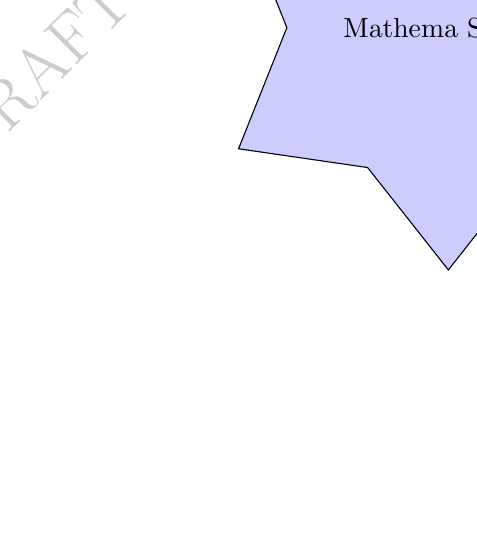
\begin{tikzpicture}
		\tikz \node [fill=blue!20,star,star points=6,draw] {Mathema Shukur };
	\end{tikzpicture}
	\\
	যাদের জন্যে প্রযোজ্যঃ  	\textcolor{magenta}{একাদশ ও দ্বাদশ শ্রেণীর শিক্ষার্থী} \\
	বিষয়ঃ \textcolor{magenta}{উচ্চতর গণিত ১ম পত্র} \\
	অধ্যায়ঃ \textcolor{magenta}{৩-সরলরেখা}\\ 
	Subtopicঃ  \textcolor{magenta}{ মূল নিয়মে ত্রিভুজের ক্ষেত্রফল নির্ণয় করা   }\\
	\\
		দিনাজপুর বোর্ড-২০১২\\ 
 দুইটি অক্ষরেখা পরস্পর লম্ব ভাবে  $O$ বিন্দুতে ছেদ করে। $A$ ও $B$ এর ধনাত্মক স্থানাঙ্ক যথাক্রমে $(x_1,y_1)$ ও $(x_2,y_2)$ ।  মূল নিয়মে প্রমাণ কর যে, ত্রিভুজটির ক্ষেত্রফল $\frac{1}{2}|x_1\,\,y_2-x_2\,\,y_1|$ বর্গ একক \\ 
	\\ 
		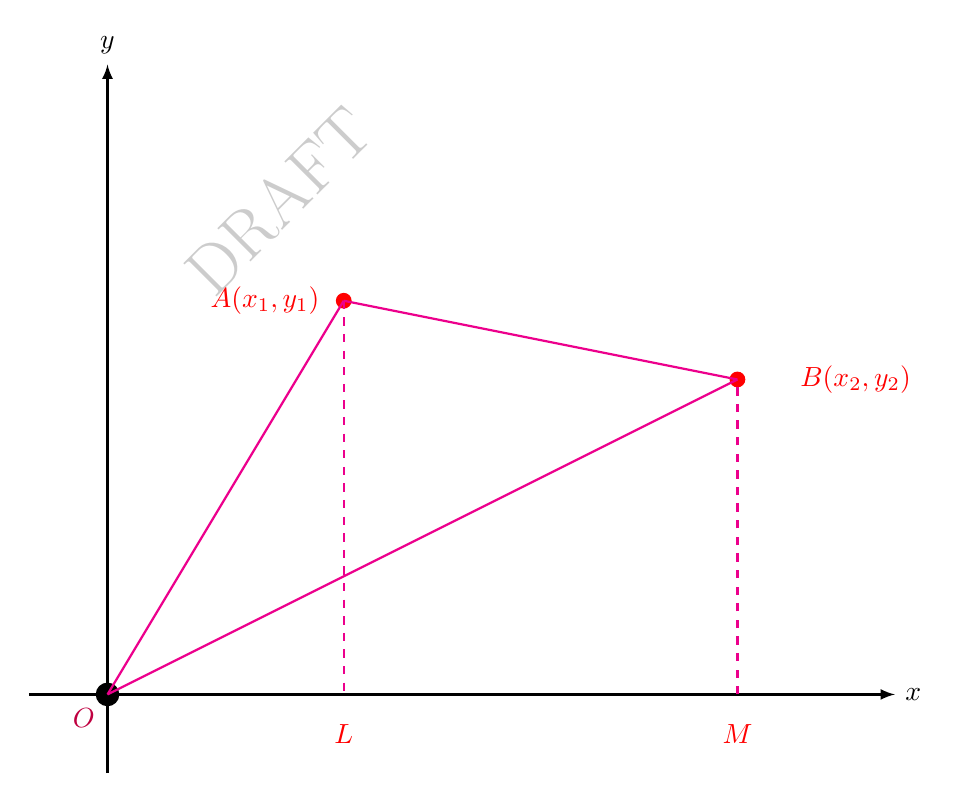
\begin{tikzpicture}[transform shape,scale=1]
		\draw [-latex,thick](-1,0) -- (10,0) node[right] {$x$} coordinate(x axis);
		\draw [-latex,thick](0,-1) -- (0,8) node[above] {$y$} coordinate(y axis);
		\fill[black] (0,0) circle (1.5 mm);
		\node at (-0.3,-0.3) {$\textcolor{purple}{O}$};	
		\fill[red] (3,5) circle (1 mm);
		\fill[red] (8,4) circle (1 mm);
		\node at (2,5) {$\textcolor{red}{A(x_1,y_1)}$};	
		\node at (9.5,4) {$\textcolor{red}{B(x_2,y_2)}$};	
			\node at (3,-0.5) {$\textcolor{red}{L}$};	
				\node at (8,-0.5) {$\textcolor{red}{M}$};			
		\draw[thick,magenta] (3,5)--(0,0);
		\draw[thick,magenta,dashed] (3,5)--(3,0);
		\draw[thick,magenta] (8,4)--(0,0);
		\draw[thick,magenta] (3,5)--(8,4);
		\draw[thick,magenta,dashed] (8,0)--(8,4);
	\end{tikzpicture}
	\\
	\vspace{3cm}
	\\
		ত্রিভুজের ক্ষেত্রফল\\
	$\frac{1}{2}\times$	ভূমি $\times$  উচ্চতা\\
\\
		\begin{tikzpicture}[transform shape,scale=1]
		\draw [-latex,thick](-1,0) -- (10,0) node[right] {$x$} coordinate(x axis);
		\draw [-latex,thick](0,-1) -- (0,8) node[above] {$y$} coordinate(y axis);
		\fill[black] (0,0) circle (1.5 mm);
		\node at (-0.3,-0.3) {$\textcolor{purple}{O}$};	
		\fill[red] (3,5) circle (1 mm);
		\node at (2,5) {$\textcolor{red}{A(x_1,y_1)}$};	
		\node at (5,3) {$\textcolor{blue}{T_{OA}=\frac{1}{2}\,\,x_1\,\,y_1}$};	
		\node at (3,-0.5) {$\textcolor{red}{L}$};			
		\draw[thick,magenta] (3,5)--(0,0);
		\draw[thick,magenta,dashed] (3,5)--(3,0);
	\end{tikzpicture}
	\\
ট্রাপিজিয়ামের ক্ষেত্রফল \\
\\ 
$\frac{1}{2}\times $(ট্রাপিজিয়ামের সমান্তরাল বাহুদ্বয়ের যোগফল) $\times$ (ট্রাপিজিয়ামের সমান্তরাল বাহুদ্বয়ের মধ্যবর্তী দূরত্ব)\\ 
\\ 
	\begin{tikzpicture}[transform shape,scale=1]
	\draw [-latex,thick](-1,0) -- (10,0) node[right] {$x$} coordinate(x axis);
	\draw [-latex,thick](0,-1) -- (0,8) node[above] {$y$} coordinate(y axis);
	\fill[black] (0,0) circle (1.5 mm);
	\node at (-0.3,-0.3) {$\textcolor{purple}{O}$};	
	\fill[red] (3,5) circle (1 mm);
	\fill[red] (8,4) circle (1 mm);
		\node at (4,7) {$\textcolor{blue}{T_{AB}=\frac{1}{2}(y_1+y_2)(x_2-x_1)}$};	
	\node at (2,5) {$\textcolor{red}{A(x_1,y_1)}$};	
	\node at (9.5,4) {$\textcolor{red}{B(x_2,y_2)}$};	
	\node at (3,-0.5) {$\textcolor{red}{L}$};	
	\node at (8,-0.5) {$\textcolor{red}{M}$};			
	\draw[thick,magenta,dashed] (3,5)--(3,0);
	\draw[thick,magenta] (3,5)--(8,4);
	\draw[thick,magenta,dashed] (8,0)--(8,4);
\end{tikzpicture}
\\
\vspace{3cm}
\\
	ত্রিভুজের ক্ষেত্রফল\\
$\frac{1}{2}\times$	ভূমি $\times$  উচ্চতা\\
\\
	\begin{tikzpicture}[transform shape,scale=1]
	\draw [-latex,thick](-1,0) -- (10,0) node[right] {$x$} coordinate(x axis);
	\draw [-latex,thick](0,-1) -- (0,8) node[above] {$y$} coordinate(y axis);
	\fill[black] (0,0) circle (1.5 mm);
	\node at (-0.3,-0.3) {$\textcolor{purple}{O}$};	
	\fill[red] (8,4) circle (1 mm);
	\node at (9.5,4) {$\textcolor{red}{B(x_2,y_2)}$};	
		\node at (5,5) {$\textcolor{cyan}{T_{OB}=\frac{1}{2}\,\,x_2\,\,y_2}$};	
	\node at (8,-0.5) {$\textcolor{red}{M}$};			
	\draw[thick,magenta] (8,4)--(0,0);
	\draw[thick,magenta,dashed] (8,0)--(8,4);
\end{tikzpicture}
\\
	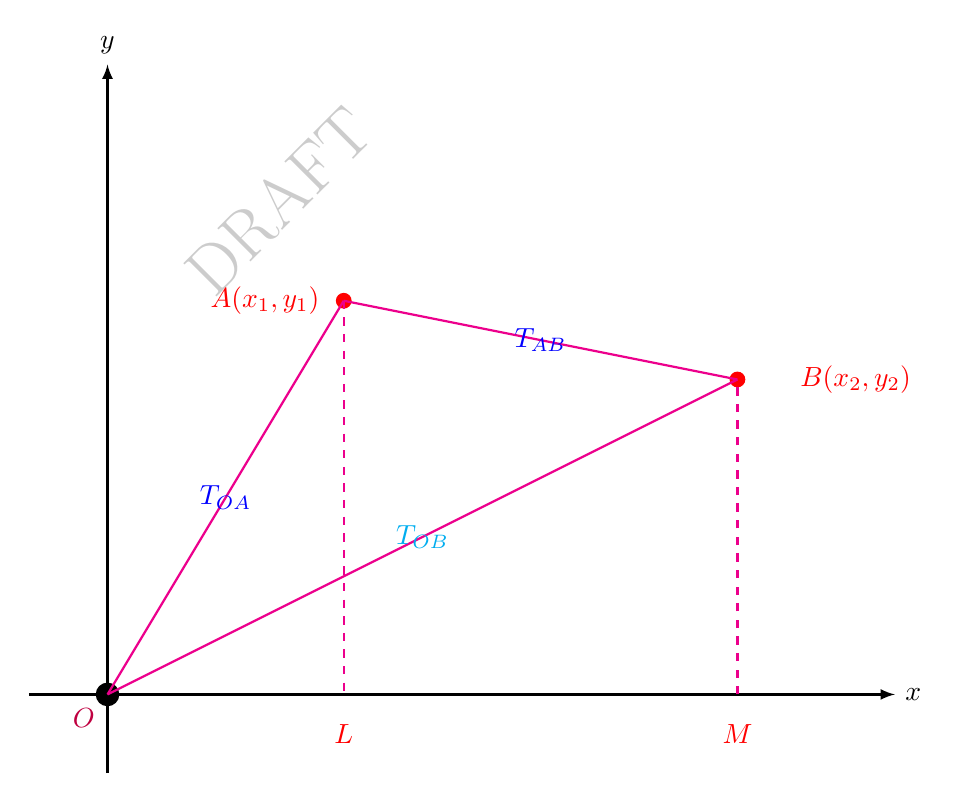
\begin{tikzpicture}[transform shape,scale=1]
	\draw [-latex,thick](-1,0) -- (10,0) node[right] {$x$} coordinate(x axis);
	\draw [-latex,thick](0,-1) -- (0,8) node[above] {$y$} coordinate(y axis);
	\fill[black] (0,0) circle (1.5 mm);
	\node at (-0.3,-0.3) {$\textcolor{purple}{O}$};	
	\fill[red] (3,5) circle (1 mm);
	\fill[red] (8,4) circle (1 mm);
	\node at (2,5) {$\textcolor{red}{A(x_1,y_1)}$};	
	\node at (9.5,4) {$\textcolor{red}{B(x_2,y_2)}$};	
	\node at (3,-0.5) {$\textcolor{red}{L}$};	
	\node at (8,-0.5) {$\textcolor{red}{M}$};			
	\draw[thick,magenta] (3,5)--(0,0);
	\draw[thick,magenta,dashed] (3,5)--(3,0);
	\draw[thick,magenta] (8,4)--(0,0);
	\draw[thick,magenta] (3,5)--(8,4);
	\draw[thick,magenta,dashed] (8,0)--(8,4);
		\node at (1.5,2.5) {$\textcolor{blue}{T_{OA}}$};	
		\node at (5.5,4.5) {$\textcolor{blue}{T_{AB}}$};
		\node at (4,2) {$\textcolor{cyan}{T_{OB}}$};
\end{tikzpicture}
\\
\begin{align*}
	\triangle AOB &= \textcolor{blue}{T_{OA}}+\textcolor{blue}{T_{AB}}-\textcolor{cyan}{T_{OB}}\\
	\\
	&=\frac{1}{2}\,\,x_1\,\,y_1+\frac{1}{2}(y_1+y_2)(x_2-x_1)-\frac{1}{2}\,\,x_2\,\,y_2\\
	\\
	&=\frac{1}{2} \left[x_1\,\,y_1+(y_1+y_2)(x_2-x_1)-x_2\,\,y_2\right]\\
	\\
	&=\frac{1}{2} (x_1\,\,y_1+x_2\,\,y_1-x_1\,\,y_1+x_2\,\,y_2-x_1\,\,y_2-x_2\,\,y_2)\\
	\\
	&=\frac{1}{2}|x_1\,\,y_2-x_2\,\,y_1|
\end{align*}
	ঢাকা বোর্ড-২০১৪\\ 
	$ABC$ ত্রিভুজের শীর্ষ বিন্দুগুলি  $A(5,6)$, $B(-9,1)$, $C(-3,-1)$ । ত্রিভুজটির ক্ষেত্রফল নির্ণয় কর । এর সাহায্যে  $A$ থেকে $BC$ এর উপর অঙ্কিত লম্বের দৈর্ঘ্য নির্ণয় কর \\
	\\  
		\begin{tikzpicture}[transform shape,scale=1]
		\draw [-latex,thick](-10,0) -- (6,0) node[right] {$x$} coordinate(x axis);
		\draw [-latex,thick](0,-3) -- (0,7) node[above] {$y$} coordinate(y axis);
		\fill[black] (0,0) circle (1.5 mm);
		\node at (-0.3,-0.3) {$\textcolor{purple}{O}$};	
		\fill[red] (5,6) circle (1 mm);
			\fill[red] (-3,-1) circle (1 mm);
		\fill[red] (-9,1) circle (1 mm);
		\node at (6,6) {$\textcolor{red}{A(5,6)}$};	
			\node at (2,-2) {$\textcolor{red}{D}$};	
		\node at (-9,1.5) {$\textcolor{red}{B(-9,1)}$};			
		\node at (-1.5,-1) {$\textcolor{red}{C(-3,-1)}$};		
		\draw[thick,magenta] (5,6)--(-3,-1);
			\draw[thick,magenta,dashed] (5,6)--(2.1,-2.9);
				\draw[thick,magenta,dashed] (-3,-1)--(2.1,-2.9);
		\draw[thick,magenta] (-9,1)--(5,6);
		\draw[thick,magenta] (-9,1)--(-3,-1);
	\end{tikzpicture}
\\
\\
$(x_1,y_1)=A(5,6)$,\quad $(x_2,y_2)=B(-9,1)$,\quad $(x_3,y_3)=C(-3,-1)$\\
\\ 
\begin{align*}
	\triangle ABC=	&\frac{1}{2}\begin{vmatrix}
		x_1 &	y_1 & 1\\
		x_2 & y_2 & 1\\
		x_3 & y_3 & 1
	\end{vmatrix}\\
	\\
	&=\frac{1}{2}\begin{vmatrix}
		5 & 6 & 1\\
		-9 & 1 & 1\\
		-3 & -1 & 1
	\end{vmatrix}\\
	&\boxed{Expansion \quad by \quad  First \quad  Column}\\ 
	&=\frac{1}{2}\left\{(5)\begin{vmatrix}
		1 & 1\\
		-1 & 1
	\end{vmatrix}-(-9)\begin{vmatrix}
		6 & 1\\
		-1 & 1
	\end{vmatrix}+(-3)\begin{vmatrix}
		6 & 1\\
		1 & 1
	\end{vmatrix}\right\}\\
	\\
	&=\frac{1}{2}\left[(5)(1+1)-(-9)(6+1)+(-3)(6-1)\right]\\
	\\
	&=\frac{1}{2}\left[10+63-15\right]\\
	\\
	\triangle ABC	&=29
\end{align*}
\\ 
	\\
ত্রিভুজের ক্ষেত্রফল\\
$\frac{1}{2}\times$	ভূমি $\times$  উচ্চতা\\
\\
\begin{align*}
	\triangle ABC &= \frac{1}{2}\times BC \times AD\\
	\\
29  &= \frac{1}{2}\times BC \times AD\\
\\
AD&= \frac{58}{BC}\qquad [\textcolor{blue}{BC=\sqrt{(-9+3)^2+(1+1)^2}=2\sqrt{10}}]\\
\\
AD&= \frac{58}{2\sqrt{10}}\\
\\
AD&= \frac{29\sqrt{10}}{10}
\end{align*}
\\
\\
\\
		কুমিল্লা বোর্ড-২০২১\\ 
	$ABC$ ত্রিভুজের শীর্ষ বিন্দুগুলি  $A(-3,-2)$, $B(-3,9)$, $C(5,-8)$ । ত্রিভুজটির ক্ষেত্রফল নির্ণয় কর । এর সাহায্যে  $B$ থেকে $CA$ এর উপর পতিত  লম্বের দৈর্ঘ্য নির্ণয় কর \\
	\\  
		\\  
	\begin{tikzpicture}[transform shape,scale=1]
		\draw [-latex,thick](-9,0) -- (6,0) node[right] {$x$} coordinate(x axis);
		\draw [-latex,thick](0,-9) -- (0,9) node[above] {$y$} coordinate(y axis);
		\fill[black] (0,0) circle (1.5 mm);
		\node at (-0.3,-0.3) {$\textcolor{purple}{O}$};	
		\fill[red] (-3,-2) circle (1 mm);
		\fill[red] (-3,9) circle (1 mm);
		\fill[red] (5,-8) circle (1 mm);
		\node at (6,-7.5) {$\textcolor{red}{C(5,-8)}$};	
		\node at (-7.5,2) {$\textcolor{red}{D}$};	
		\node at (-3,9.5) {$\textcolor{red}{B(-3,9)}$};			
		\node at (-4,-2.5) {$\textcolor{red}{A(-3,-2)}$};		
		\draw[thick,magenta] (-3,9)--(-3,-2);
			\draw[thick,magenta,dashed] (-3,9)--(-8.5,2);
		\draw[thick,magenta] (-3,9)--(5,-8);
		\draw[thick,magenta] (5,-8)--(-3,-2);
			\draw[thick,magenta,dashed] (-8.5,2)--(-3,-2);		
	\end{tikzpicture}
	\\
	( DO IT YOURSELF) \\ 
	\\
	$\triangle ABC=44$,\qquad $BD=8\frac{4}{5}$\\
	\\ 
		বরিশাল বোর্ড-২০০৫\\ 
	$ABC$ ত্রিভুজের শীর্ষ বিন্দুগুলি  $A(3,5)$, $B(-3,3)$, $C(-1,-1)$ । $D,\,\,E,\,\,F$ যথাক্রমে  $BC,\,\,CA,\,\,AB$ এর মধ্যবিন্দু ।  $\triangle ABC$ ও  $\triangle DEF$ এর ক্ষেত্রফল নির্ণয় কর । দেখাও যে  $\triangle ABC= 4\triangle DEF$\\ 
	\\ 
	\\
	\\
	 $B(-3,3)$, ও $C(-1,-1)$ এর মধ্যবিন্দু হচ্ছে  $D\left(\frac{-3-1}{2},\frac{3-1}{2}\right)=D(-2,1)$\\
	 \\
	 $C(-1,-1)$, ও  $A(3,5)$ এর মধ্যবিন্দু হচ্ছে  $E\left(\frac{3-1}{2},\frac{5-1}{2}\right)=E(1,2)$\\
	 \\
	 $A(3,5)$, ও  $B(-3,3)$ এর মধ্যবিন্দু হচ্ছে  $F\left(\frac{3-3}{2},\frac{5+3}{2}\right)=F(0,4)$\\
	 \\ 
		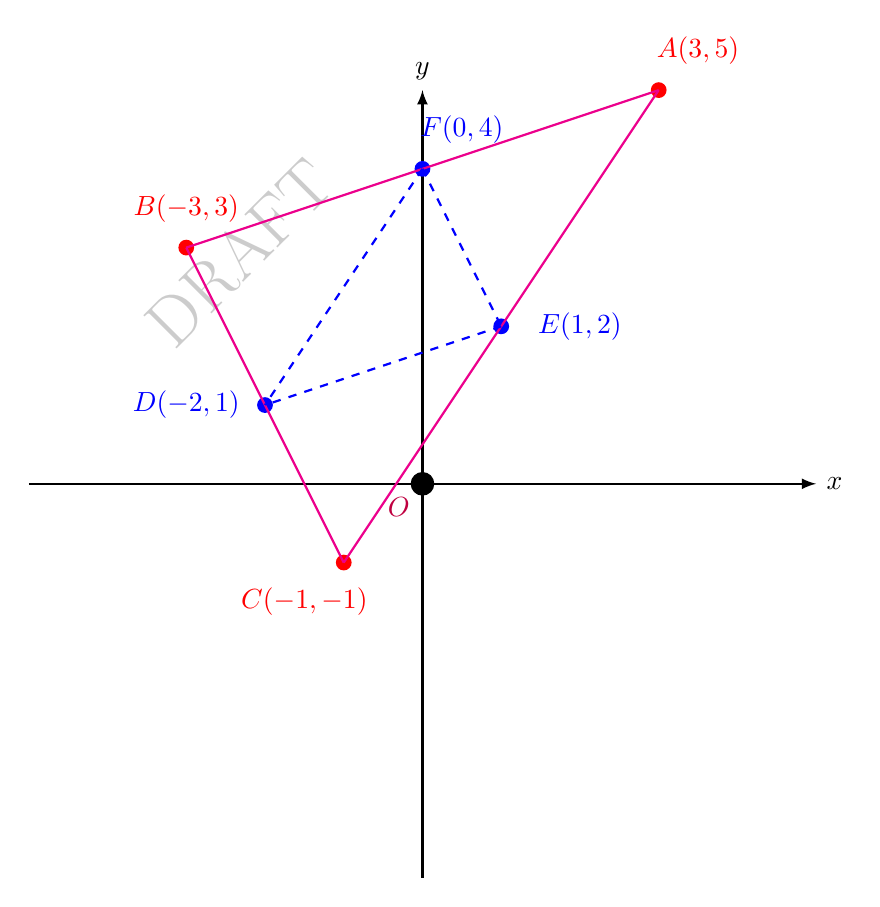
\begin{tikzpicture}[transform shape,scale=1]
		\draw [-latex,thick](-5,0) -- (5,0) node[right] {$x$} coordinate(x axis);
		\draw [-latex,thick](0,-5) -- (0,5) node[above] {$y$} coordinate(y axis);
		\fill[black] (0,0) circle (1.5 mm);
		\node at (-0.3,-0.3) {$\textcolor{purple}{O}$};	
		\fill[red] (3,5) circle (1 mm);
		\fill[red] (-3,3) circle (1 mm);
		\fill[red] (-1,-1) circle (1 mm);
			\fill[blue] (0,4) circle (1 mm);
		\fill[blue] (1,2) circle (1 mm);
		\fill[blue] (-2,1) circle (1 mm);
		\node at (-1.5,-1.5) {$\textcolor{red}{C(-1,-1)}$};	
		\node at (-3,3.5) {$\textcolor{red}{B(-3,3)}$};			
		\node at (3.5,5.5) {$\textcolor{red}{A(3,5)}$};		
		\draw[thick,magenta] (3,5)--(-3,3);
		\draw[thick,magenta] (3,5)--(-1,-1);
		\draw[thick,magenta] (-3,3)--(-1,-1);
			\node at (-3,1) {$\textcolor{blue}{D(-2,1)}$};	
		\node at (2,2) {$\textcolor{blue}{E(1,2)}$};			
		\node at (0.5,4.5) {$\textcolor{blue}{F(0,4)}$};			
			\draw[thick,blue,dashed] (0,4)--(1,2);	
				\draw[thick,blue,dashed] (0,4)--(-2,1);	
						\draw[thick,blue,dashed] (1,2)--(-2,1);	
	\end{tikzpicture}
	\\
	\begin{align*}
		\triangle ABC &=\frac{1}{2}\begin{vmatrix}
			3 & 5 & 1\\
			-3 & 3 & 1\\
			-1 & -1 & 1
		\end{vmatrix}\\
		&\boxed{Expansion \quad by \quad  First \quad  Column}\\ 
		&=\frac{1}{2}\left\{(3)\begin{vmatrix}
			3 & 1\\
			-1 & 1
		\end{vmatrix}-(-3)\begin{vmatrix}
			5 & 1\\
			-1 & 1
		\end{vmatrix}+(-1)\begin{vmatrix}
			5 & 1\\
			3 & 1
		\end{vmatrix}\right\}\\
		\\
		&=\frac{1}{2}\left[(3)(3+1)-(-3)(5+1)+(-1)(5-3)\right]\\
		\\
		&=\frac{1}{2}\left[12+18-2\right]\\
		\\
		\triangle ABC	&=14
	\end{align*}
\\
	\begin{align*}
	\triangle DEF &=\frac{1}{2}\begin{vmatrix}
		-2 & 1 & 1\\
		1 & 2 & 1\\
		0 & 4 & 1
	\end{vmatrix}\\
	&\boxed{Expansion \quad by \quad  First \quad  Column}\\ 
	&=\frac{1}{2}\left\{(-2)\begin{vmatrix}
		2 & 1\\
		4 & 1
	\end{vmatrix}-(1)\begin{vmatrix}
		1 & 1\\
		4 & 1
	\end{vmatrix}+(0)\begin{vmatrix}
		1 & 1\\
		2 & 1
	\end{vmatrix}\right\}\\
	\\
	&=\frac{1}{2}\left[(-2)(2-4)-(1-4)+0\right]\\
	\\
	&=\frac{1}{2}\left[4+3\right]\\
	\\
	\triangle DEF	&=\frac{7}{2}
\end{align*}
\\
\begin{align*}
	\triangle ABC &=14\\
	\\
\triangle ABC &=4\times \frac{7}{2}\\
	\\
\triangle ABC &=4\times \triangle DEF\\
\end{align*}
\\
	BUET-2001-2002\\
	$ABC$ ত্রিভুজের মধ্যমাগুলির মধ্যবিন্দু  $(1,2)$, $(4,4)$ এবং $(2,8)$; ত্রিভুজটির ক্ষেত্রফল নির্ণয় কর \\
	\\
	ধরি, মধ্যমাগুলির  মধ্য বিন্দু দ্বারা গঠিত ত্রিভুজটি $\triangle DEF$\\
	\\ 
		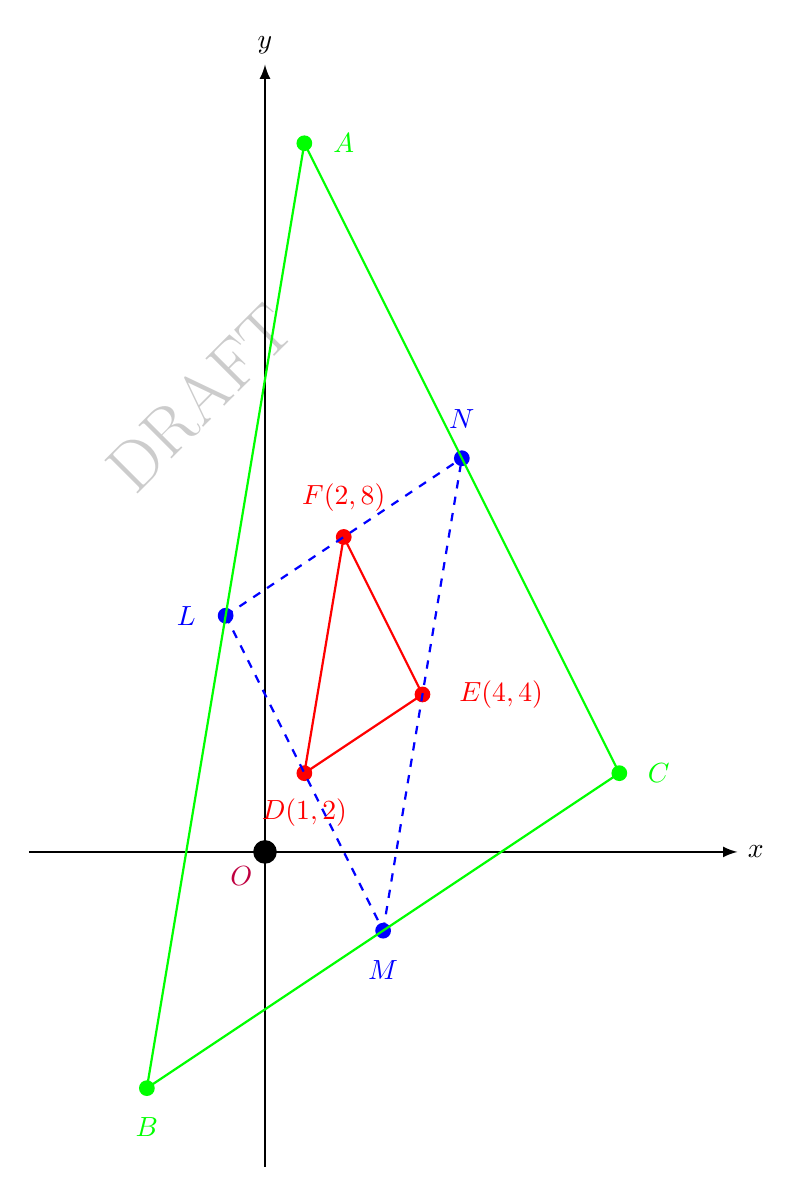
\begin{tikzpicture}[transform shape,scale=1]
		\draw [-latex,thick](-3,0) -- (6,0) node[right] {$x$} coordinate(x axis);
		\draw [-latex,thick](0,-4) -- (0,10) node[above] {$y$} coordinate(y axis);
		\fill[black] (0,0) circle (1.5 mm);
		\node at (-0.3,-0.3) {$\textcolor{purple}{O}$};	
		\fill[red] (0.5,1) circle (1 mm);
		\fill[red] (2,2) circle (1 mm);
			\fill[red] (1,4) circle (1 mm);	
		\draw[thick,red] (0.5,1)--(2,2);
		\draw[thick,red] (0.5,1)--(1,4);
		\draw[thick,red] (2,2)--(1,4);
			\node at (0.5,0.5) {$\textcolor{red}{D(1,2)}$};	
		\node at (3,2) {$\textcolor{red}{E(4,4)}$};			
		\node at (1,4.5) {$\textcolor{red}{F(2,8)}$};	
			\fill[blue] (-0.5,3) circle (1 mm);
		\fill[blue] (1.5,-1) circle (1 mm);
		\fill[blue] (2.5,5) circle (1 mm);	
		\draw[thick,blue,dashed] (-0.5,3)--(1.5,-1);
		\draw[thick,blue,dashed] (-0.5,3)--(2.5,5);
		\draw[thick,blue,dashed] (1.5,-1)--(2.5,5);
			\node at (-1,3) {$\textcolor{blue}{L}$};	
		\node at (1.5,-1.5) {$\textcolor{blue}{M}$};			
		\node at (2.5,5.5) {$\textcolor{blue}{N}$};	
			\fill[green] (0.5,9) circle (1 mm);
		\fill[green] (-1.5,-3) circle (1 mm);
		\fill[green] (4.5,1) circle (1 mm);	
		\draw[thick,green] (0.5,9)--(-1.5,-3);
		\draw[thick,green] (0.5,9)--(4.5,1);
		\draw[thick,green] (4.5,1)--(-1.5,-3);
			\node at (1,9) {$\textcolor{green}{A}$};	
		\node at (-1.5,-3.5) {$\textcolor{green}{B}$};			
		\node at (5,1) {$\textcolor{green}{C}$};	
	\end{tikzpicture}
\\
		\begin{align*}
		\triangle DEF &=\frac{1}{2}\begin{vmatrix}
			1 & 2 & 1\\
			4 & 4 & 1\\
			2 & 8 & 1
		\end{vmatrix}\\
		&\boxed{Expansion \quad by \quad  First \quad  Column}\\ 
		&=\frac{1}{2}\left\{(1)\begin{vmatrix}
			4 & 1\\
			8 & 1
		\end{vmatrix}-(4)\begin{vmatrix}
			2 & 1\\
			8 & 1
		\end{vmatrix}+(2)\begin{vmatrix}
			2 & 1\\
			4 & 1
		\end{vmatrix}\right\}\\
		\\
		&=\frac{1}{2}\left[(4-8)-(4)(2-8)+(2)(2-4)\right]\\
		\\
		&=\frac{1}{2}\left[-4+24-4\right]\\
		\\
		\triangle DEF	&=8\\
	\end{align*}
\begin{multicols}{2}
	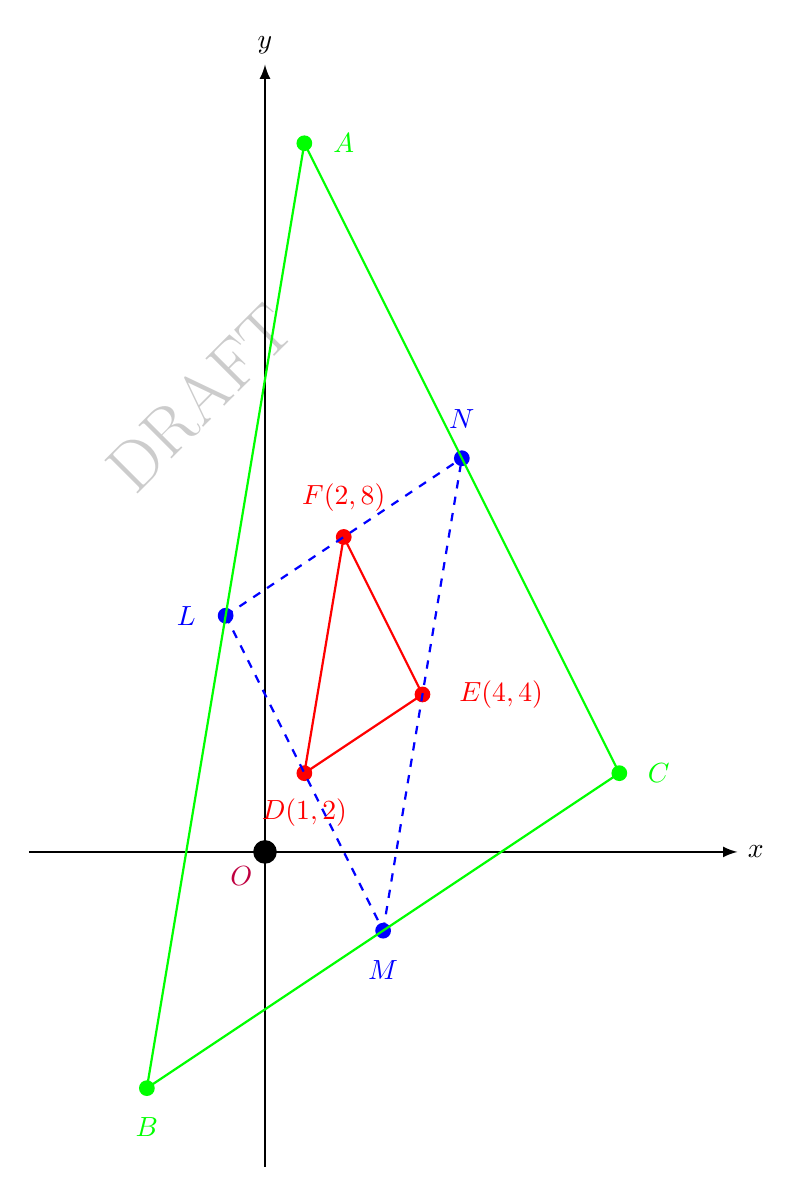
\begin{tikzpicture}[transform shape,scale=1]
	\draw [-latex,thick](-3,0) -- (6,0) node[right] {$x$} coordinate(x axis);
	\draw [-latex,thick](0,-4) -- (0,10) node[above] {$y$} coordinate(y axis);
	\fill[black] (0,0) circle (1.5 mm);
	\node at (-0.3,-0.3) {$\textcolor{purple}{O}$};	
	\fill[red] (0.5,1) circle (1 mm);
	\fill[red] (2,2) circle (1 mm);
	\fill[red] (1,4) circle (1 mm);	
	\draw[thick,red] (0.5,1)--(2,2);
	\draw[thick,red] (0.5,1)--(1,4);
	\draw[thick,red] (2,2)--(1,4);
	\node at (0.5,0.5) {$\textcolor{red}{D(1,2)}$};	
	\node at (3,2) {$\textcolor{red}{E(4,4)}$};			
	\node at (1,4.5) {$\textcolor{red}{F(2,8)}$};	
	\fill[blue] (-0.5,3) circle (1 mm);
	\fill[blue] (1.5,-1) circle (1 mm);
	\fill[blue] (2.5,5) circle (1 mm);	
	\draw[thick,blue,dashed] (-0.5,3)--(1.5,-1);
	\draw[thick,blue,dashed] (-0.5,3)--(2.5,5);
	\draw[thick,blue,dashed] (1.5,-1)--(2.5,5);
	\node at (-1,3) {$\textcolor{blue}{L}$};	
	\node at (1.5,-1.5) {$\textcolor{blue}{M}$};			
	\node at (2.5,5.5) {$\textcolor{blue}{N}$};	
	\fill[green] (0.5,9) circle (1 mm);
	\fill[green] (-1.5,-3) circle (1 mm);
	\fill[green] (4.5,1) circle (1 mm);	
	\draw[thick,green] (0.5,9)--(-1.5,-3);
	\draw[thick,green] (0.5,9)--(4.5,1);
	\draw[thick,green] (4.5,1)--(-1.5,-3);
	\node at (1,9) {$\textcolor{green}{A}$};	
	\node at (-1.5,-3.5) {$\textcolor{green}{B}$};			
	\node at (5,1) {$\textcolor{green}{C}$};	
\end{tikzpicture}
\\
\begin{align*}
	\triangle ABC &=4\times \triangle LMN\\
	\\
	\triangle ABC &=4\times 4\times DEF\\
	\\
	\triangle ABC &=16\times DEF\\
	\\
	\triangle ABC &=16\times 8\\ 
	\\
	\triangle ABC &=128\\ 
\end{align*}
\end{multicols}
\end{document}